This section discusses the mathematical and algorithmic concepts of a 2D graph
representation and its relevance for MMIR. We have introduced Graph Codes in [22]. They
are applicable to any kind of feature graph, but we specifically designed them for MMIR.
They should provide a huge benefit in the area or multimedia indexing and retrieval as a
technical representation basis for graph algorithms. We use them to represent MMFGs and
to transform these into another mathematical space for fast and efficient MMIR.
Our Graph Code Encoding algorithm [22] uses the Valuation Matrix VM of a given
MMFG as a basis. It is also possible to calculate Graph Codes based on n-dimensional
vector-spaces and a projection of these into a 2D matrix-space, producing a similar result
as the algorithm based on the Valuation Matrix. We chose to employ Valuation Matrices,
as this approach is expected to require fewer calculations than vector-space transformations.

% Beispiel eines MMFGs ... gibts bereits im MMFG Abschnitt... Verweisen

% Übergehen zur Wertungsmatrix

In general, the graph encoding algorithm receives a graph structure as input—in our
case, a MMFVG.

Graph codes are a solid basis for ML, as there are already many training
models for pattern matching and deviation detection.

Graph Codes [2,33] are a 2D projection of a multimedia feature graph based on adjacency matrix operations [34], where the feature vocabulary terms of a feature graph are presented by row and column indices, and matrix positions represent relationships between these features. It has been demonstrated that Graph Codes are efficient for similarity and
recommendation searches, as they basically use linear growing matrix operations instead of exponentially growing graph-traversal-based algorithms.

Graph Codes contain a dictionary dictGC of feature vocabulary terms FVT (i.e., the row and column descriptions) and represent the relationships between dictionary terms as value of a matrix field mi,j. As Graph Codes represent multidimensional MMIR features, a similarity metric triple MGC = (MF,MFR,MRT) has been defined, containing a featuremetric MF based on the vocabulary, a feature-relationship-metric MFR based on the possible relationships, and a feature-relationship-type-metric MRT based on the actual relationship types. This similarity metric can be applied for the calculation of MMIR results.

This section discusses the mathematical and algorithmic concepts of a 2D graph representation and its relevance for MMIR. We have introduced Graph Codes in [22]. They are applicable to any kind of feature graph, but we specifically designed them for MMIR. They should provide a huge benefit in the area or multimedia indexing and retrieval as a technical representation basis for graph algorithms. We use them to represent MMFGs and to transform these into another mathematical space for fast and efficient MMIR. Our Graph Code Encoding algorithm [22] uses the Valuation Matrix VM of a given MMFG as a basis. It is also possible to calculate Graph Codes based on n-dimensional vector-spaces and a projection of these into a 2D matrix-space, producing a similar result as the algorithm based on the Valuation Matrix. We chose to employ Valuation Matrices, as this approach is expected to require fewer calculations than vector-space transformations.


Valuation Matrices contain one row and column for each node, always resulting in
square matrices. Edges incident on nodes n1 and n2 are represented in the matrix with
their weight or a value of 1 at row n1 and column n2, i.e., position (n1, n2). In case of
the example above, the set of nodes N is given by N = {Person, Head, Human Being,
Individual, Hat, above}, represented by a value of 1 in one of the diagonals of the matrix.
Thus, the Valuation Matrix VM is defined as (see also Table 1 and Figure 3):

Valuation Matrices contain one row and column for each node, always resulting in
square matrices. Edges incident on nodes n1 and n2 are represented in the matrix with their
weight or a value of 1 at row n1 and column n2, i.e., position (n1, n2). In case of the above
example, the set of nodes N is given by N = {Person, Head, Human Being, Individual, Hat,
above}, represented by a value of 1 in one of the diagonals of the matrix. Thus, the Valuation

Graph Codes employ a encoding function fenc, which calculates a numeric value for
each non-zero position of a Valuation Matrix based on node or edge type and the corresponding attributes. The function fenc can be adjusted deliberately to meet the requirements
of any application. In the context of this paper, we chose an arbitrary selection of value
ranges representing type attributes of nodes and edges for the Graph Code representation.
If we apply such a fenc to the above example (object-node = 1, synonym-node = 2, childrelationship = 3, synonym-relationship = 4, relationship = 5, spacial-relationship-node = 6),
the encoded Valuation Matrix VMenc i.e., the corresponding Graph Code GC is shown in
Figure 4 and Table 2, where node representing fields are painted in bold. Node types in
Table 2 are coloured according to Figure 1 and represented by the fields in the diagonal of
the matrix. Edge types are coloured (3 = orange, 4 = purple, 5 = yellow)

In future encodings, attributes, weights, or other information about nodes and edges
can be encoded with more complex functions resulting in arbitrary natural numbers. In our
model, we apply the encoding function fenc to each matrix field and base it on e.g., threebyte-
integer values between 0 and 16.7 million (=maxc in the later equations). The reason
for this is that the resulting Graph Codes can then be interpreted as bitmap images,
which provides some benefits in visualization during testing, evaluating, and manually
proving results. Although in general, fenc can be arbitrary defined according to the MMIR
application’s requirements.

Here, we will introduce the definitions for vocabularies, their dictionaries, and therefore
feature term vocabulary representations of Graph Codes. Based on these definitions,
a metric for similarity calculations going beyond node and edge types, based on Graph
Codes can be defined. Summarizing our current example, matrices can represent only node
and edge types so far. In each MMFG, the set of n nodes representing distinct feature terms
can be regarded as unique identifiers for the MMFG’s feature term vocabulary FVTMMFG:
FVTMMFG = f f t1, . . . , f tng (4)
This set of a MMFG’s vocabulary terms thus represents the elements of a corresponding
Graph Code’s Dictionary, i.e., the set of all individual feature vocabulary terms of a

Graph Code. However, it is important to uniquely identify the feature vocabulary term
assigned to a field of a Graph Code. Thus, we introduce a Graph Code Dictionary for
each Graph Code, which is represented by a vector dictGC and provides a ordered representation
of the set FVTMMFG with uniquely defined positions for each MMFG’s feature
vocabulary term. The elements in dictGC can be ordered according to the corresponding
MMFG, e.g., by applying a breadth-first-search, but also other ordering strategies could be
applied. As the ordering does not effect the Graph Code algorithms and concepts as such,
in the following examples, we chose a manual ordering to maximize illustration. In the
Graph Code matrix representation, each node field (in the diagonal) of a Graph Code can
now be unambiguously mapped to an entry of its Graph Code Dictionary vector, which
can be represented as follows:
dictGC = ( f t1, . . . , f tn) (5)
Applied to the Graph Code of the previous example, the set of feature vocabulary
terms FVTex would be {Person, Head, Human Being, Individual, Hat, above}, in which the
elements do not have any order. The corresponding vector dictex would be:
dictex = (Person, Head, HumanBeing,
Individual, Hat, above)
and—in contrast to the set representation—uniquely identifies each vocabulary term by its
position within the vector. Thus, dictex can also be regarded as a indexed list:

When comparing the similarity of two Graph Codes, it is important to compare
only feature-equivalent node fields in the diagonal of each matrix to each other. Each
Graph Code has its own, individual dictionary-vector dictGC, and another Graph Code
will have a different dictionary-vector according to the content of its represented MMFG,
typically dictGC1 6= dictGC2. Feature-equivalent node fields of Graph Codes can be determined
through their corresponding Graph Code Dictionaries, as these fields will have
positions represented by an equal feature vocabulary term of each corresponding dictionary.
For comparison, only the set of intersecting feature vocabulary terms of e.g., two
Graph Codes is relevant, as non-intersecting feature vocabulary terms would represent
non-common MMFG feature nodes, which cannot be similar. Thus, the set of intersecting
feature vocabulary terms FVT1,2 of e.g., two MMFGs can be defined as:
FVT1,2 = f f t1, . . . , f tng = VMMFVG1 \ VMMFVG2 (6)
The methodology of intersecting sets can be also applied to Graph Code dictionaries.
The intersection of two vectors dict1, 2 can be defined correspondingly as:
dict1,2 = dictGC1 \ dictGC2 (7)
To illustrate the calculation of dict\, we introduce a second exemplary Graph Code
GCex2 based on a MMFGex2 as shown in Figure 5 and the corresponding Table 3.

The set FVTex2 in this case is above, Dog, Head, Animal, Hat and the set FTV1,2 of
intersecting feature vocabulary terms is above, Head, Hat. The dictionary-vector dictex2
thus is:
dictex2 = (above, Dog, Head, Animal, Hat)
illustrated as a indexed list, dictex2 would be:
Index i 1 2 3 4 5
f ti above Dog Head Animal Hat
The vector dictex1,2 represents the dictionary of intersecting vocabulary terms and
only contains the subset of vocabulary terms of dictex, where a equal vocabulary term can
be found in dictex2. The order of intersecting vocabulary terms in dict1,2 is given by the
order of dictex:
dictex1,2 = (above, Head, Hat)
From an algorithmic perspective, this means that all elements of dictex are deleted that
cannot be found in dictex2. Typically, the index position of dict1,2 is different from both
dict1 and dict2. For our example, the indexed list representation of dictex1,2 would be:
Index i 1 2 3
f ti above Head Hat
Based on these dictionary-vectors, a translation of equivalent Graph Code positions
can be performed, as each feature vocabulary term has a unique position within each of
the Graph Code’s dictionaries.
Applications will typically utilize a collection of MMFGs and their corresponding
Graph Codes. The overall feature term vocabulary FVTColl = f f t1, . . . , f tcg containing
c vocabulary terms of such a collection of n MMFGs can be defined as the union of all
MMFG’s feature term vocabularies and also be represented by the union of all Graph Code
Dictionaries dict[:
FVTColl =
[n
i=1
FVTMMFGi (8)
8i, j < n : dict[ = dicti  dictj (9)
In this dict[ dictionary-union-vector, the -operation for calculating the union of
dictionary-vectors is implemented by traversing all the collection’s dicti dictionaries and
collecting unique dictionary vocabulary terms into a single dictionary-vector. In case of
our example with dictex and dictex2, the calculated dict[ = (Person, Head, Human Being,



Die Berechnung von $dict_{\cap}$ wird im Folgenden auf Basis eines zweiten MMFGs $MMFG_{ex_2}$, abgebildet in \cref{sec2:sota:subsec:fz-explainablity:fig:mmfg-example-2}, demonstriert.

\begin{figure}[htb]
    \centering
    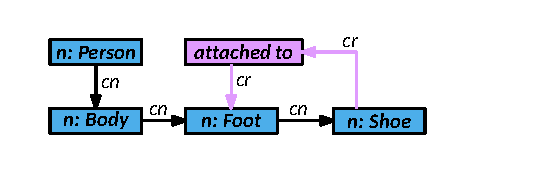
\includegraphics[width=0.7\textwidth]{chapter/chapter_2/mmfg-ex2.eps}
    \caption{Beispiel für einen $MMFG_{ex_2}$.}
    \label{sec2:sota:subsec:fz-explainablity:fig:mmfg-example-2}
\end{figure}
%Die Menge an Bezeichnern für das Beispiel $MMFG_{ex_2}$ ist $FVT_{ex_2} = \{Person,Body,Foot,Shoe,attached~to\}$ und die Schnittmenge für beide Mengen an Bezeichnern beider Beispiele ist $FVT_{1 \cap 2} = \{Person,Body,attached~to\}$.
%Das Wörterbuch ist $dict_{ex_2} = (attached~to,Person,Body,Foot,Shoe)$.

\begin{table}[htb]
    \centering
    \begin{tabular}{rcccccc}
         &  \begin{turn}{90}attached to\end{turn}& \begin{turn}{90}Person\end{turn} & \begin{turn}{90}Body\end{turn} & \begin{turn}{90}Foot\end{turn} & \begin{turn}{90}Shoe\end{turn} \\ \hline
        attached to      & \cellcolor{comprel}6 & 0 & 0 & \cellcolor{comprel}5 & 0  \\ 
        Person           & 0 & \cellcolor{nodeblue}1 & \cellcolor{nodeblue}3 & 0 & 0  \\
        Body             & 0 & 0 & \cellcolor{nodeblue}1 & \cellcolor{nodeblue}3 & 0  \\ 
        Foot             & 0 & 0 & 0 & \cellcolor{nodeblue}1 & \cellcolor{nodeblue}3  \\ 
        Shoe             & \cellcolor{comprel}5 & 0 & 0 & 0 & \cellcolor{nodeblue}1           
    \end{tabular}
    \caption{T}
    \label{tab:my_label}
\end{table}

\begin{table}[htb]
    \centering
    \begin{tabular}{c|c|c|c|c|c}
        Index $i$ & 1 & 2 & 3 & 4 & 5 \\ \hline
        $fvt_i$ & attached to & Person & Body & Foot & Shoe
    \end{tabular}
    \caption{Caption}
    \label{tab:my_label}
\end{table}